\documentclass[a4paper,11pt]{scrartcl}

\usepackage{graphicx}
\usepackage[utf8]{inputenc} 
\usepackage{amsmath,amssymb,amsthm} 
\usepackage[round]{natbib}
\usepackage{url}
\usepackage{xspace}
\usepackage[left=20mm,top=20mm]{geometry}
\usepackage{algorithmic}
\usepackage{subcaption}
\usepackage{mathpazo}
\usepackage{booktabs}
\usepackage{hyperref}
% \usepackage{draftwatermark}

\newcommand{\ie}{ie}
\newcommand{\eg}{eg}
\newcommand{\reffig}[1]{Figure~\ref{#1}}
\newcommand{\refsec}[1]{Section~\ref{#1}}

\setcapindent{1em} %-- for captions of Figures

\renewcommand{\algorithmicrequire}{\textbf{Input:}}
\renewcommand{\algorithmicensure}{\textbf{Output:}}


\title{Documentation Notes}
\date{}
\author{Giuseppe Cervone\\ \url{giuseppe.cervone@edu.unife.it}}

\begin{document}

\maketitle

\section{Introduction}
The aim of the project is to develop what in cybersecurity and IoT is called a data diode, a unidirectional communication device for data exchange. The importance behind this project is that industrial data diodes are expensive devices, and implementing a high amount of them like for this specific use case is a very costly move, but with software implementations (firewalls) or hardware implementations (serial or optical communications) it is possible to have cheaper data diodes that are almost as functional for most use case scenario. The setup will include two Raspberry Pi model 3 with a specific configuration which we will highlight later, and a TTL-232R-3V3 cable without the RX pin being plugged in one of the raspberries.

\section{Devices}
\subsection{Raspberry Pi}
As far as the Raspberry Pi models, I have chosen to use the Raspberry Pi 3 as it's a nice midway point between performance and cost. This particular machine should be able to handle the data size we are planning to share (around 1Gb/day), at a cost that is much lower than that of a Raspberry Pi 4. The machines are configured as follows:
\begin{itemize}
    \item Raspberry Pi 3 Model B Ver1.2:
    \begin{itemize}
        \item Quad Core 1.2GHz Broadcom BCM2837 64bit CPU
        \item 1GB RAM
        \item BCM43438 wireless LAN and Bluetooth Low Energy (BLE) on board
        \item 100 Base Ethernet
        \item 40-pin extended GPIO
        \item 4 USB 2 ports
        \item 4 Pole stereo output and composite video port
        \item Full size HDMI
        \item CSI camera port for connecting a Raspberry Pi camera
        \item DSI display port for connecting a Raspberry Pi touchscreen display
        \item Micro SD port for loading your operating system and storing data
        \item Upgraded switched Micro USB power source up to 2.5A
        \item Raspberry Pi OS Lite (latest version)
        \item 16GB microSD card
    \end{itemize}
\end{itemize}

Using the RPI-Imager tool I installed the latest Raspberry PI OS image. Upon first boot up, remember that raspberry pi login is username: pi, password: raspberry. As Raspberry Pi OS Lite is an OS without a desktop environment, so we can use raspi-config to enable a series of features useful for testing software:
\begin{itemize}    
    \item In the system options:
    \begin{itemize}
        \item Enable WIFI.
        \item Change username and password if needed.
    \end{itemize}
    \item In the interface options:
    \begin{itemize}
        \item Enable SSH.
        \item Enable Serial interface, remembering to disable login shell but enable serial interface.
    \end{itemize}
    \item Run sudo apt-get upgrade to make sure all packages are up to date before using raspi-config.
    \item Disable bluetooth:
        \begin{itemize}
            \item We won't be using bluetooth for the project, so we disable it, making the final product more secure.
            \item We disable bluetooth by adding 'dtoverlay=disable-bt' in /boot/config.txt.
        \end{itemize}
    \item Troubleshooting
        \begin{itemize}
            \item Check that UART is enabled in /boot/config.txt by adding 'enable\_UART=1'.
            \item Check that serial console is disabled by removing "console=serial0,115200" (or "console=ttyS0,115200") in /boot/cmdline.txt.
            \item Check for permissions in the dialout group.
            \item Check that /dev/serial0 doesn't have a getty console running on it. In case it does, it can be disabled by using the commands: sudo systemctl stop serial-getty@ttyS0.service and sudo systemctl disable serial-getty@ttyS0.service.
        \end{itemize}
\end{itemize}

\subsection{UART Cable}
As mentioned earlier, the serial communication will go through a TTL-232R-3V3 cable, which is USB to UART, with +3.3V TTL levels UART signals. The cable has 3-pins on one end, and USB on the other. Using GPIO14 pin on the RPi we can trasmit data, using GPIO15 we receive data. As previously mentioned, GPIO15 can be removed after the initial tests are over, as the communication will be one-way. In appendix 1, we can see an extract from the the documentation of the cable, showing the correct way to plug in the cable in the correct pins. With the cable plugged in we run the command ls /dev/tty* on both raspberry machines so we have an idea of what port we are using on each raspberry in the serial communication (For the port that's sending data it should be /dev/ttyS0, while for the other port it should be USB0). Raspian will always map the serial port to /dev/serial0, so it is suggested to use the alias in programming. In Appendix 2 is an image of how the two machines should look like once plugged in. This image also gives us further information on which machine will be exposed to a future outside network, and which machine won't have communications coming in.

\section{First test}
Having the machines setup, you can test if the machines are working correctly by running the two programs found in appendix 1. In case this program won't run correctly, refer back to the troubleshooting section earlier. The code sndtest.py has to be run on the machine where the GPIO pins are being used, and recvtest.py has to be run on the machine where the USB is plugged in. It's suggested you start by running recvtest.py using the command python3 recvtest.py, and then run python3 sndtest.py. Below is an image of what it should look like. (Aggiungero' in futuro, sono sulle raspberry)

\section{Data diode 0.1}
The first implementation of a data diode I will try out is a project based on a github repo that is not mantained anymore. https://github.com/thephez/data-diode. (Da ampliare)

\section{Appendix}
\subsection{Appendix 1: Pinout uart}
\begin{figure}[htbp]
\centerline{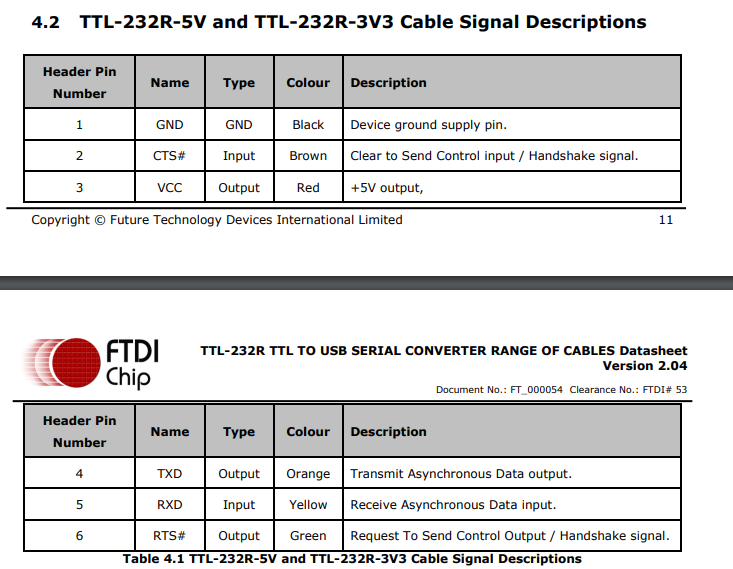
\includegraphics{pinout uart.png}}
\caption{Pinout del cavo seriale}
\label{fig2}
\end{figure}

\subsection{Appendix 2: Machines plugged in}
\begin{figure}[htbp]
\centerline{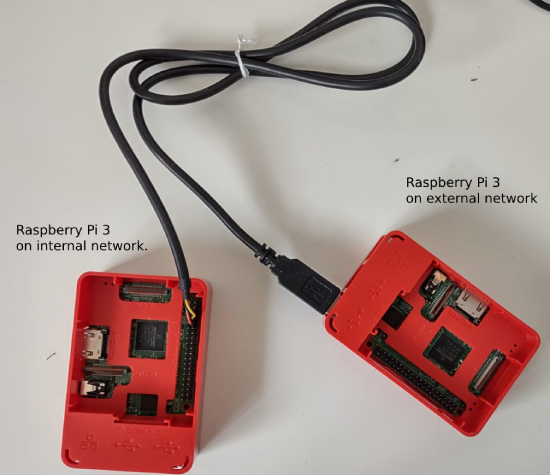
\includegraphics{0.0.1.png}}
\caption{Example 1}
\label{fig}
\end{figure}

\subsection{Appendix 3: Example code and output}

\bibliographystyle{plainnat}
\bibliography{/Users/hugo/references/references}
\end{document}
